\chapter{A Reintroduction to Areal Co\"ordinates}

\textbf{Benedict Randall Shaw}

\begin{multicols}{2}

Several issues ago, an article was published in this publication with the title \say{An Introduction to Areal Co\"ordinates}. Regrettably, having revisited this article, it seems to have been below the usual standard, and worryingly cursory. However, the topic itself is of use and interest; thus, this article is intended to do that which the original failed to, viz. introduce the reader to areal co\"ordinates.

This article is aimed at those who wish to do vaguely well in olympiads, but find themselves unable to do geometry by Euclidean (normal) methods. While most olympiad questions are designed to be done by such methods, there exist other ways of doing geometry problems. Areal co\"ordinates are an example of such a method; they constitute a co\"ordinate system, in the same way that Cartesian co\"ordinates (those with which most people are most familiar) are a co\"ordinate system. They are not always successful, but tend to be useful in problems where a triangle is the central object involved.

In order to become competent with mathematic concepts, it is helpful to practise; so, throughout this article I shall leave questions that can be done by those wishing to become competent.

\fbox{Such questions will be placed in boxes, thus.}

\end{multicols}
\section{Definitions}
\begin{multicols}{2}

We say that a point anywhere in the plane \(P\) has co\"ordinates \((x,y,z)\) with respect to a triangle \(\triangle{}ABC\) iff \[(x,y,z)=\left(\frac{[PBC]}{[ABC]},\frac{[APC]}{[ABC]},\frac{[ABP]}{[ABC]}\right)\] where \([DEF]\), for some triangle \(DEF\), is the area of \(\triangle{}DEF\).

\end{multicols}

\begin{figure}[h]
	\centering
	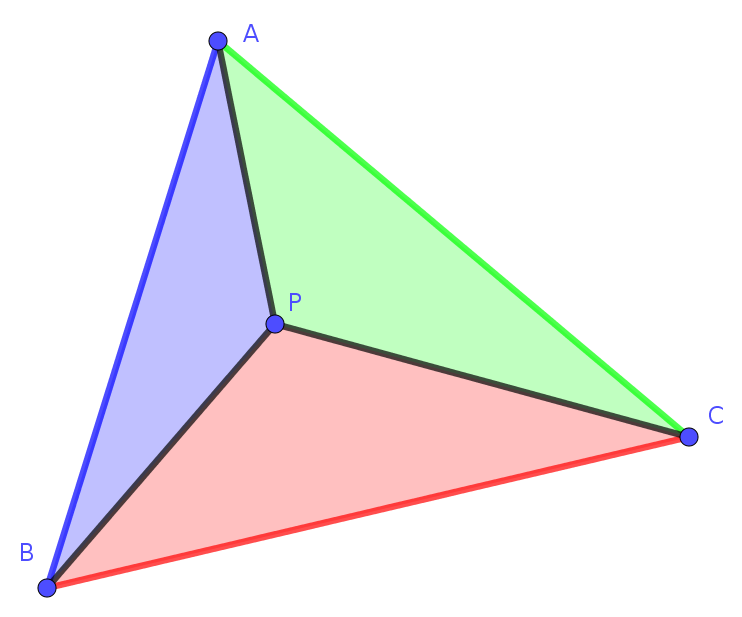
\includegraphics[width=0.5\linewidth]{def-areas}
	\caption{A point \(P\), with respect to \(\triangle{}ABC\).}
	\label{def-areas}
\end{figure}

\begin{multicols}{2}

Note that \(x+y+z=1\) is thus always true, as clearly \([PBC]+[APC]+[ABP]\). We thus have a rigorously defined unique set of co\"ordinates for all points within the triangle. But what about those outside the triangle? First, we must define directed areas. When we name a triangle, convention says that we label its points anticlockwise. We therefore say that \([ABC]\) is positive if \(A,B,C\) are in order going anticlockwise around \(\triangle{}ABC\), and negative if the points are in order going clockwise. (If the points \(A,B,C\) are in a straight line, then \([ABC]\) is obviously zero.) We now have a distinct set of co\"ordinate for all points in the plane. \fbox{Prove this.}

An equivalent definition exists with vectors. For any arbitrary point \(O\) in the plane, point \(P\) has co\"ordinates \((x,y,z)\) with respect to \(\triangle{}ABC\) iff \(\overrightarrow{OP}=x\overrightarrow{OA}+y\overrightarrow{OB}+z\overrightarrow{OC}\) and \(x+y+z=1\). It does not matter where we choose \(O\); we get the same set of co\"ordinates for \(P\) whereever \(O\) is. \fbox{Prove this.}

\begin{center}
\fbox{\parbox{0.96\linewidth}{Prove that these two definitions, in terms of areas and vectors are equivalent; that is to say, all points have the same co\"ordinates under both definitions.}}\\
\end{center}

For the physically minded, there is also yet another definition; \((x,y,z)\) is the point that is the centre of mass when one places masses \(x,y,z\) at points \(A,B,C\) respectively, such that \(x+y+z=1\). Note that we allow negative masses.

It is clear that \(A,B,C\) have co\"ordinates \((1,0,0),(0,1,0),(0,0,1)\) respectively; from consideration of the definition involving areas, one can see that a point is within the triangle if and only iff all its co\"ordinates are positive.

Often we don't care about the constraint \(x+y+z=1\), and so we relax it; there is no single standard notation for this of which this correspondent is aware, so in this article, we shall use \((x,y,z)^*\) to denote \((\frac{x}{x+y+z},\frac{y}{x+y+z},\frac{z}{x+y+z})\). These are sometimes referred to as unnormalised co\"ordinates.

\end{multicols}
\section{Triangle centres}
\begin{multicols}{2}

Triangles do not have an obviously defined centre; as a result, there are numerous points known as \textit{triangle centres}, to the point where they have an encyclop\ae{}dia, which at time of writing contains 15888 centres, and is imaginatively named the \textit{Encyclopedia of Triangle Centers} (it is admittedly American). Needless to say, most of these are completely useless; however, the centres are loosely sorted by importance, and the encyclop\ae{}dia gives the areal co\"ordinates of the earlier centres, although it calls them barycentrics. Here are some important centres, and their co\"ordinates with respect to \(\triangle{}ABC\) (when they are the centres of the \(\triangle{}ABC\)). \(a,b,c\) refer to the lengths of sides \(BC,CA,AB\) respectively, and \(A,B,C\) refer to angles \(\angle{}CAB,\angle{}ABC,\angle{}BCA\) respectively.

\paragraph{Incentre} This is the centre of the incircle (the circle within the triangle tangent to all three sides) and also the intersection of the internal angle bisectors of the triangle; it has co\"ordinates \((a,b,c)^*\).

\paragraph{Centroid} This is the intersection of the medians of the triangle (the lines from vertices of the triangle to midpoints of the opposing sides); it has co\"ordinates \((1,1,1)^*\).

\paragraph{Circumcentre} This is the centre of the circle passing through all three vertices of the triangle, and the intersection of the perpendicular bisectors of the sides; it has co\"ordinates \((\sin{}2A,\sin{}2B,\sin{}2C)^*\).

\paragraph{Orthocentre} This is the intersection of the altitudes of the triangle (the perpendiculars from the vertices to the opposing sides); it has co\"ordinates \((\tan{}A,\tan{}B,\tan{}C)^*\).

\begin{center}
\fbox{\parbox{0.96\linewidth}{Prove that these are the correct co\"ordinates for the four triangle centres mentioned, whatever the triangle.}}
\end{center}

These four points are often sufficient; there are many theorems involving them, and they appear frequently in olympiads. Other points, and their co\"ordinates, can be found in the \textit{Encyclopedia of Triangle Centers}.
\end{multicols}
\section{Lines}
\begin{multicols}{2}
In the same way that the general equation for a line in Cartesian co\"ordinates is \(lx+my+c=0\) (where \(l,m,c\) are constants that are not all zero), the general equation for a line in areal co\"ordinates is \(lx+my+nz=0\) (where \(l,m,n\) are constants that are not all zero), in addition to the standard \(x+y+z=1\) required by areals. Note that this equation still works if we relax the \(x+y+z=1\) constraint and use unnormalised co\"ordinates, as scaling \(lx+my+nz\) by a constant still gives 0 for a point that is on the line.

The equation of a line through two points \((x_p,y_p,z_p)\) and \((x_q,y_q,z_q)\) is expressed most readably with a matrix determinant. For those unaware of them, matrices are rectangular arrays of numbers. We define the determinant (written with vertical lines around a matrix) of a two by two matrix thus---
\[\begin{vmatrix}a&b\\c&d\end{vmatrix}\equiv{}ad-bc\]

We define the determinant of a three by three matrix thus---
\[\begin{vmatrix}a&b&c\\d&e&f\\g&h&i\end{vmatrix}\equiv{}g\begin{vmatrix}b&c\\e&f\end{vmatrix}+h\begin{vmatrix}c&a\\f&d\end{vmatrix}+i\begin{vmatrix}a&b\\d&e\end{vmatrix}\]

The equation for a line through points \((x_p,y_p,z_p)\) and \((x_q,y_q,z_q)\) is given by this equation---
\[\begin{vmatrix}x_p&y_p&z_p\\x_q&y_q&z_q\\x&y&z\end{vmatrix}=0\]

Note that a line \(lx+my+nz=0\) passes through \(A\) iff \(l=0\), \(B\) iff \(m=0\), and \(C\) iff \(n=0\). This is fairly apparent from consideration of the co\"ordinates of the vertices. Note that if two of the co\"efficients are zero, then the line must be one of the sides of \(\triangle{}ABC\). \fbox{Prove this.}
\end{multicols}
\clearpage
\section{Areas}
\begin{multicols}{2}
For points \(P,Q,R\) with co\"ordinates  \((x_p,y_p,z_p),(x_q,y_q,z_q),\\(x_r,y_r,z_r)\), the area of \(\triangle{}PQR\) (which we denote \([PQR]\)) is given by this formula---

\[
[PQR]=[ABC]\begin{vmatrix}x_p&y_p&z_p\\x_q&y_q&z_q\\x_r&y_r&z_r\end{vmatrix}
\]

This should sound reasonable, based on the determinant definition of a line through two points; it is clear that \([PQR]=0\) iff \(P,Q,R\) are collinear, so \(R\) lies on line \(PQ\) iff the determinant has value zero.

Note that this formula clearly does not work for unnormalised co\"ordinates.

This is often enough to solve olympiad problems, along with some trigonometric competence.
\end{multicols}
\section{Circles}
\begin{multicols}{2}
Where \(a,b,c=|BC|,|CA|,|AB|\), the \textit{circumcircle} of \(\triangle{}ABC\) (the circle going through all three points \(A,B,C\)) is given by the equation \(a^2yz+b^2zx+c^2xy=0\). In fact, the general equation for a circle is given by \(a^2yz+b^2zx+c^2xy+lx+my+nz=0\), when we are using the constraint \(x+y+z=1\). If we relax that and use unnormalised co\"ordinates, we have the slightly more complex equation \(a^2yz+b^2zx+c^2xy+(x+y+z)(lx+my+nz)=0\).

For a circle in the plane passing through three points, we can find its equation by substituting the three points into the general equation and finding \(l,m,n\).
\end{multicols}
\section{Vectors \& Distances}
\begin{multicols}{2}
For those who are unaware of what a vector is, a vector denotes a specific geometric translation; that is to say, it denotes a way to move a point to another. For example, in Cartesian co\"ordinates, \[\begin{bmatrix}3\\-2\end{bmatrix}\] is the vector that denotes moving a point or other object to the right by three units and down by two units; that is to say, it is the vector that would move \((0,0)\) to \((3,-2)\). In Cartesian co\"ordinates, the vector that would take \((x_p,y_p)\) to \((x_q,y_q)\) is  \[\begin{bmatrix}x_q-x_p\\y_q-y_p\end{bmatrix}\]
\textsl{}
In Cartesian co\"ordinates, we notate vectors differently to points, as there is no way to tell them apart if we write them the same way. In areals, this is not necessary, as will become clear. The vector taking \((x_p,y_p,z_p)\) to \((x_q,y_q,z_q)\) is \((x_q-x_p,y_q-y_p,z_q-z_p)\). We need not write the vector as a column, because the sum of the values in a vector is 0, as it is the sum of the co\"ordinates of one point minus the sum of those of another. It is thus easy to differentiate vectors and points. Note that when working with vectors in areals, we cannot use unnormalised co\"ordinates.

The length of a given line segment \(PQ\), where the vector taking \(P\) to \(Q\) (or vice versa) is \((u,v,w)\), can be found from this equation--- \[-PQ^2=a^2vw+b^2wu+c^2uv\]
which is reminiscent of the formula for circles, which should seem fairly natural given the usual definition of a circle as the set of all points which are a given distance from the centre.
\end{multicols}
\section{Disclaimer}
\begin{multicols}{2}
Ideally, one ought not to use areals, as the vast majority of geometric problems have neater, more satisfying, and easier solutions using standard Euclidean methods. However, if one is unable to use those effectively for some reason, and has tried and failed to rectify this, then areals are a possible alternative; one must, however, practise using them if one wishes to use them properly and efficiently. Note that there exist other ways of doing geometry aside from areals and Euclidean methods, including but not limited to vectors, trigonometry, complex numbers, and (although this is not recommended, and is usually unhelpful) origami.
\end{multicols}